\documentclass{article}
\usepackage{graphicx}
\usepackage{hyperref}
\usepackage{listings}

\begin{document}

\begin{titlepage}

\begin{figure}[t]
\centering

\includegraphics[scale=1]{osdl-logo.png}
\end{figure}

\centering
\huge
Open Source Development Labs \\
Database Test 3 \\
Decision Support for Ad Hoc Queries \\
\huge
User's Guide \\
\large
Version 1.10

\begin{figure}[b]
\flushleft
\normalsize
Open Source Development Labs, Inc. \\
12725 SW Millikan Way, Suite 400 \\
Beaverton, OR 97005 \\
Phone: (503) 626-2455 \\
Fax: (503) 626-2436 \\
Email: info@osdl.org
\end{figure}

\end{titlepage}

\noindent
Copyright (c) 2002 by The Open Source Development Laboratory, Inc. This
material may be distributed only subject to the terms and conditions set forth
in the Open Publication License, v1.0 or later (the latest version is currently
available at \url{http://www.opencontent.org/openpub/}). Distribution of
substantively modified versions of this document is prohibited without the
explicit permission of the copyright holder.

\noindent
Other company, product or service names may be trademarks or service marks of
others.

\noindent
Contributors to this white paper include: \\
\indent Jenny Zhang (OSDL) \\
\indent Mary Edie Meredith (OSDL) \\
\indent Mark Wong (OSDL) \\

\pagebreak

\tableofcontents

\section{Introduction}

This document provides instructions on how to set up and use the
Open Source Development Lab's Database Test 3
(OSDL-DBT-3) kit.  This kit provides what is needed to execute a
workload similar to the TPC-H workload using PostgreSQL, MySQL, and MariaDB.

\subsubsection{Query Templates}

The TPC-H DBGEN tool kit includes the official query syntax for TPC-H
queries.  The tester can substitute OSDL-DBT-3 queries with TPC-H
queries and alter the syntax to fit other databases.  A set of query
syntax for SAP DB, PostgreSQL, MySQL, and MariaDB are included in the kit in the directory
dbt3/queries.  Some of the queries are modified for database specific syntax.

\section{Setup}

This section covers the steps of getting and installing the OSDL-DBT-3 test kit source code.

\subsection{Getting and Installing the Kit}

\subsection{Required Software}

In addition to the DBMS software, the following is also required:
\begin{itemize}
\item bc \url{http://www.gnu.org/software/bc/bc.html}
\item R \url{http://www.r-project.org/}
\item sar, pidstat \url{http://pagesperso-orange.fr/sebastien.godard/}\footnote{While the scripts assume this particular version of \texttt{sar} and \texttt{pidstat}, it is possible to run on non-Linux based operating systems with some modifications to the kit.}
\end{itemize}

\subsubsection{OSDL-DBT-3 Test Kit Source}

The latest stable version of the kit can be found on SourceForge
via: \url{http://sourceforge.net/project/showfiles.php?group\_id=52479}

The latest development version of the kit can be checked out using git:
\lstset{language=sh}
\begin{lstlisting}
git clone git://git.code.sf.net/p/osdldbt/dbt3
\end{lstlisting}

\subsubsection{Building the kit}

The configure script needs to be run with the specific DBMS to build qgen and dbgen.  These programs were developed to be build for specific databases at compile time.  Otherwise the rest of the scripts installed by the kit do not need to be reinstalled or recreated if a different DBMS is used.

For MySQL and MariaDB:
\lstset{language=sh}
\begin{lstlisting}
./configure --with-mysql
\end{lstlisting}

For PostgreSQL:
\lstset{language=sh}
\begin{lstlisting}
./configure --with-postgresql
\end{lstlisting}

Once the configure script has been run, the kit is built and installed by:
\begin{lstlisting}
make
make install
\end{lstlisting}

\subsubsection{Sizing the System}

A OpenOffice spreadsheet, \texttt{dbt3\_sizing.sxc}, is provided to aid in sizing the
database under the respective database directory in \textit{doc} directory of the kit.

The parameter Scale Factor can be found under the Performance tab.
The scale factor can actually be any decimal number (like 1.1 or 50)
so that if the tester wishes, the tester can create a database whose
size is not one of the officially permitted scale factors.  This
might be desirable for development purposes.  Any results should be
advertised with the scale factor used, since the performance varies
based on the amount of data required for processing the queries.  The
database size is defined with reference to scale factor.  For
example, for scale factor 1, the raw data files' total size is roughly 1 GB.

Note:  This kit does not support scale factors less than 1.  Although
you can build a database using scale factors less than 1, the query
generator (qgen) will not generate the proper variable values that
correspond to scale factors less than 1.

The data displayed under the database size tab report the expected
size of the database, for the parameters entered, are to be used for
the physical database layout.  The number to note is the total number
of 8 KB pages since SAP DB uses those units in most of its
configuration settings.  Keep in mind that additional space must be
added to account for auxiliary structures such as indexes, temporary
tables and 1\% for inserts.

The tester needs to allocate space for the flat files generated by
dbgen used to load the database.  Under the tab database size, one column Flat File Size is provided to calculate the
space.  Once the database is loaded and backed up, there is no need
to retain these flat files.  

\section{Running the Test Kit}

\subsubsection{Setting OSDL-DBT-3 Environment Variables}

The dbgen, qgen and OSDL-DBT-3 scripts require specific environment variables to be set in order to function properly.
The following environment variables are required to be set and there are examples provides
in the examples directory:
\begin{itemize}
\item \textbf{DSS\_PATH=/tmp/dss\_path} - Absolute path in which to build flat files.
\item \textbf{DSS\_QUERY=/tmp/dbt3/queries/pgsql} - Absolute path in which to find
      query templates, this example is for the PostgreSQL templates.
\item \textbf{DSS\_CONFIG=/tmp/dbt3/src/dbgen} - directory in which to find
      configuration files.
\end{itemize}

Testers can choose to run all the tests in OSDL-DBT-3 as well as part
of the tests.  The following section describes how to run all the
tests in OSDL-DBT-3.

Tester may also create several databases so that several scale
factors can be tested or various implementation strategies compared.
They will only need to change environment variables to point to the
correct database as described in Section 2.2 prior to executing the
test kit scripts.

Each DBMS may have additional environment variables that need to be set.  The following sections details the required variables.

\subsubsection{MySQL/MariaDB Environment Variables}

\begin{itemize}
\item \textbf{DBNAME=dbt3} - This is the database name to use.
\item \textbf{MYDATA=/tmp/mydata} - This defines where to initialize the MySQL data directory
\end{itemize}

\subsubsection{PostgreSQL Environment Variables}

\begin{itemize}
\item \textbf{PGDATABASE=dbt3} - This is the database name to use.
\item \textbf{PGDATA=/tmp/pgdata} - This defines where the PostgreSQL instance will be created.
\item \textbf{DEFAULT\_LOAD\_PARAMETERS=``-c shared\_buffers=1GB''} - This defines the database parameters to be set for the load test.  The syntax is that same as that used to set parameters from the command line as if using \texttt{pg\_ctl}. (e.g. "-c shared\_buffers=1GB")
\item \textbf{DEFAULT\_POWER\_PARAMETERS=``''} - This defines the database parameters to set for the power test.
\item \textbf{DEFAULT\_THROUGHPUT\_PARAMETERS=``''} - This defines the database parameters to be set for the throughput test.
\end{itemize}

\subsection{Quick Start}

Only one command needs to be issued to run a complete test:
\lstset{language=sh}
\begin{lstlisting}
dbt3-run-workload -a pgsql -f 1 -o /tmp/results
\end{lstlisting}

This will run the generate the data files for a 1GB scale factor database load, power and throughput test, with 1 stream, against PostgreSQL and record the results of the test in \textit{/tmp/results}.

The \texttt{dbt3-run-workload} script can be used to run any combination of a load test, power test, and throughput test.  A load tests must be run in order to create the database before a power or throughput tests can be run individually.

\subsubsection{Addition PostgreSQL execution notes}

There is an addition \textit{-e} flag that can be used for testing PostgreSQL, which will execute the queries in the power and throughput tests using \textbf{EXPLAIN (ANALYZE, BUFFERS)} instead of returning the query results.

\section{Test Results}

The results directory, as specified when running the \texttt{dbt3-run-workload-scripts} by the \textit{-o} option, will contain the calculated metrics of the test as well as charts of the system and database statistics summarized in the \texttt{index.html} file in the results directory.

The query results chart display the execute time of each query for the power test, and the arithmetic mean of each of the streams in the throughput test.

\begin{center}
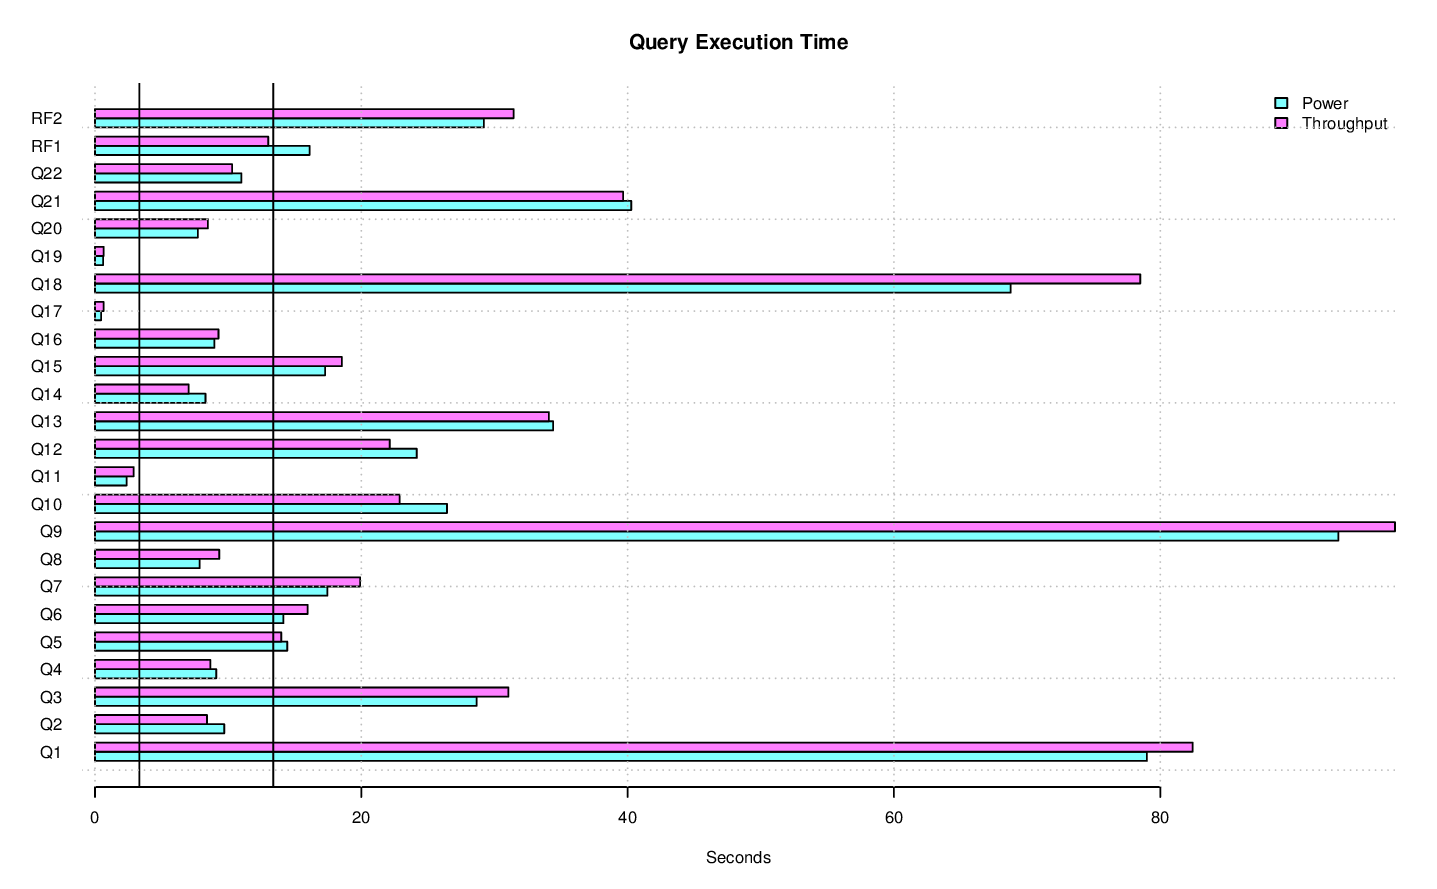
\includegraphics[scale=0.5]{q_time.png}
\end{center}

The links to the load test, power test, and throughput test summaries will have links to processor and disk utilization charts as well as operating system and database parameters used in each test.  The power test and throughput test will also have links to the query plans and query results.

\section{Tips \& Tricks}

\subsection{Linux perf tool}

The scripts assume that the kernel address maps are not restricted if the Linux
perf tool is used.  To make sure they are unrestricted, set the Linux kernel
parameter to zero by:

\lstset{language=sh}
\begin{lstlisting}
echo 0 > /proc/sys/kernel/kptr_restrict
echo -1 > /proc/sys/kernel/perf_event_paranoid
\end{lstlisting}

or editing \texttt{/etc/sysctl.conf} with:
\lstset{language=sh}
\begin{lstlisting}
kernel.kptr_restrict = 0
kernel.perf_event_paranoid = -1
\end{lstlisting}

then as \textbf{root} run:
\lstset{language=sh}
\begin{lstlisting}
sysctl -p
\end{lstlisting}

\subsection{QGEN}

The \texttt{qgen} program can be manually run to inspect the SQL statement to that will be executed by the test.

For example (see \texttt{qgen -h} for option descriptions) to see what the first query to be executed:
\lstset{language=sh}
\begin{lstlisting}
qgen -c -r 0 -p 0 -s 1 5
\end{lstlisting}

Results in the following query for PostgreSQL.
\lstset{language=sql}
\begin{lstlisting}
-- using 0 as a seed to the RNG
-- @(#)14.sql	2.1.8.1
-- TPC-H/TPC-R Promotion Effect Query (Q14)
-- Functional Query Definition
-- Approved February 1998
BEGIN;



select
	100.00 * sum(case
		when p_type like 'PROMO%'
			then l_extendedprice * (1 - l_discount)
		else 0
	end) / sum(l_extendedprice * (1 - l_discount)) as promo_revenue
from
	lineitem,
	part
where
	l_partkey = p_partkey
	and l_shipdate >= date '1993-01-01'
	and l_shipdate < cast(date '1993-01-01' + interval '1 month' as date);
COMMIT;
\end{lstlisting}

\end{document}
